\section{Engineering Components}
\label{s:eng}

\subsection{Software Engineering}
\label{ss:se}

\paragraph{Requirements elicitation.}
Requirements were elicited from three sources: brainstorming within the team (inputs, outputs, and how users can trust the output); instructor feedback on the proposal, which stressed that evaluation must work without a domain expert and that the scope must be explicit; and a peer review by another project group. The peer review raised six points. Three were already covered (command-line commands, prompt templates, legal disclaimer). Two led to new requirements: warnings for operational failures such as API quota limits and low-confidence verification (FR11), and input hardening against malformed files and prompt injection (a security non-functional requirement). One revealed that reviewers still assumed the vector-retrieval design of our proposal, which prompted us to explain the simplified v1 design more clearly (Section~\ref{ss:changes}).

\paragraph{Requirements.}
Figure~\ref{fig:fr} shows how the core functional requirements link together. The system accepts a project description (FR1) and/or a dependency manifest (FR2); looks up each dependency's license (FR3); recommends exactly three licenses from the catalogue (FR4); explains each with plain-language claims that cite a clause (FR5); verifies every claim (FR6); flags conflicting and unknown dependency licenses (FR7); asks clarifying questions when input is vague (FR8); and shows the quoted clause as evidence (FR9). Peer review added a command-line interface (FR10) and operational warnings (FR11). The main non-functional requirements are \emph{faithfulness} (never mark a false claim as verified; target precision $\geq 0.9$), \emph{transparency} (every claim links to its source clause), \emph{safety} (a ``not legal advice'' disclaimer on every result), \emph{cost} (run on a free API tier plus a local verifier), \emph{privacy} (manifests are never stored), \emph{security and robustness} (file type, size, and parsing checks; inputs treated as untrusted), and \emph{reproducibility} (seeded, versioned data and scripts). We prioritised FR1/FR2, FR4, FR5, FR6, and faithfulness as the top five.

\begin{figure*}[tb]
    \centering
    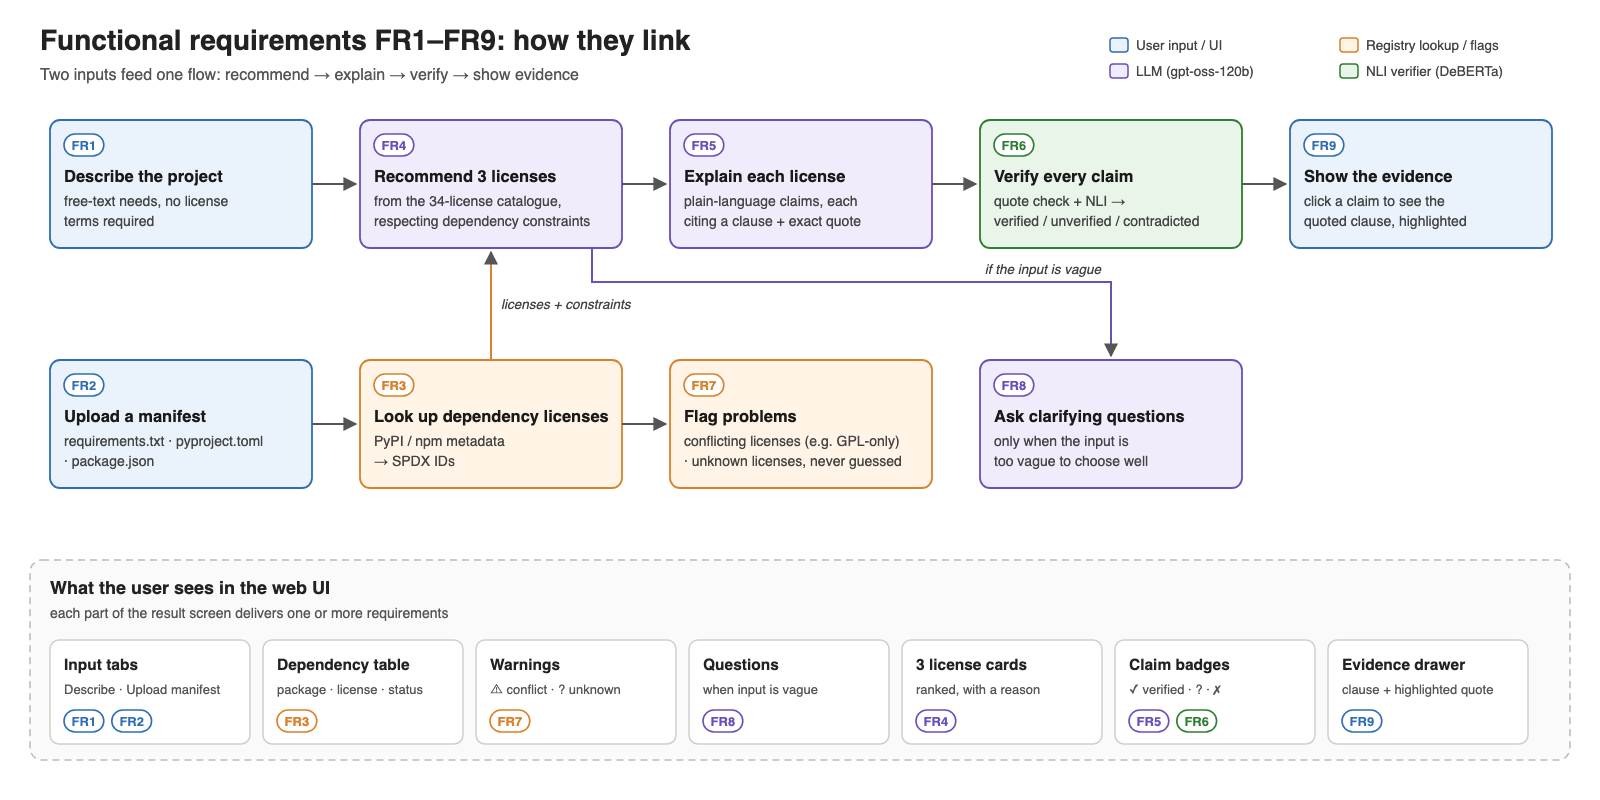
\includegraphics[width=0.92\textwidth]{13_functional_requirements.png}
    \caption{Functional requirements FR1--FR9 and how they link: two inputs feed one flow (recommend, explain, verify, show evidence); the bottom strip shows where each requirement appears in the user interface.}
    \label{fig:fr}
\end{figure*}

\paragraph{Architecture.}
Figure~\ref{fig:arch} shows the architecture. A React web UI sends requests to a FastAPI backend that runs the \texttt{licensewise} pipeline as a background job, because a request takes one to five minutes on the free API tier; the UI polls for the result. The pipeline has seven steps: (1) input validation; (2) dependency license lookup from PyPI or npm metadata, normalised to SPDX identifiers, with unrecognised licenses flagged as \emph{unknown} rather than guessed; (3) Stage~1, in which the LLM infers the developer's requirements and recommends exactly three licenses from the catalogue; (4) clause retrieval, which selects only the clauses of each license that express its obligations; (5) Stage~2, in which the LLM writes three to five claims per license, each citing one clause and quoting it verbatim; (6) NLI verification; and (7) response building. Offline components build the knowledge base and run the evaluation harness, which calls the same pipeline in batch.

\begin{figure*}[tb]
    \centering
    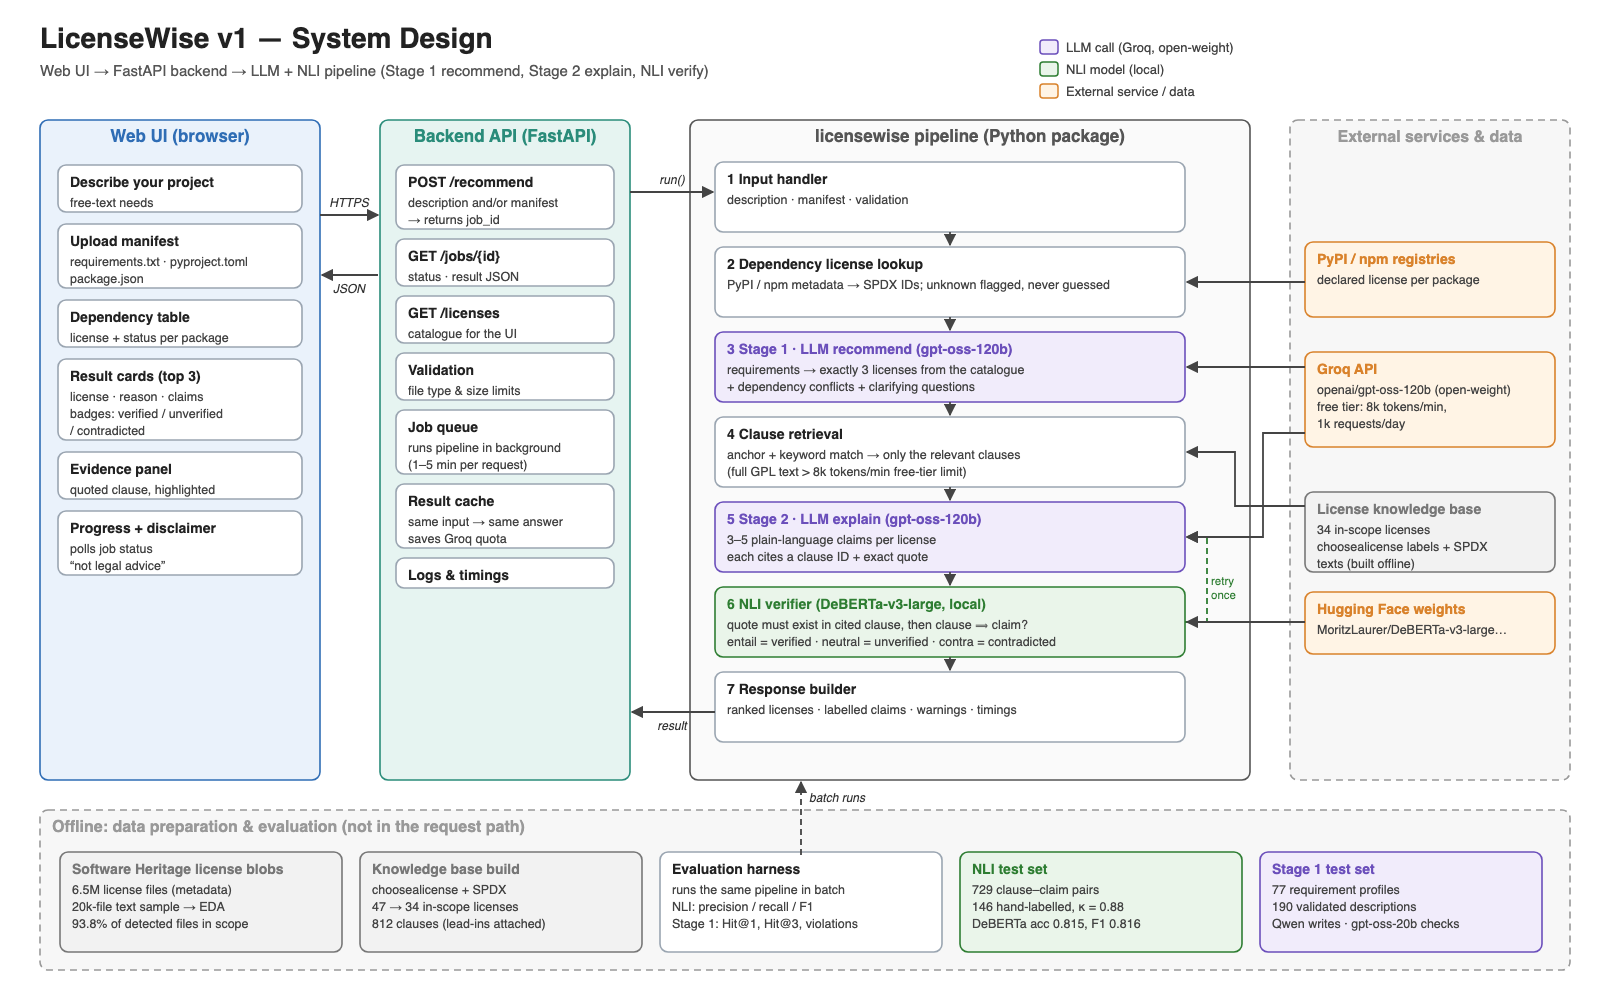
\includegraphics[width=\textwidth]{system_design.png}
    \caption{System design: web UI, FastAPI backend, and the seven-step LLM\,+\,NLI pipeline, with external services and the offline data-preparation and evaluation components.}
    \label{fig:arch}
\end{figure*}

\paragraph{User interface.}
Figure~\ref{fig:ui} shows the four-step user flow in the web interface: the developer describes the project (or uploads a manifest), the pipeline panel shows each step as it completes, the results show three license cards whose claims carry status badges, and selecting a claim opens the cited clause with the quoted words highlighted, together with the verifier's probabilities. Status badges always combine an icon with a text label, so status is never conveyed by colour alone. The UI is complete but not yet connected to the backend; it currently displays saved outputs of the real pipeline.

\begin{figure*}[tb]
    \centering
    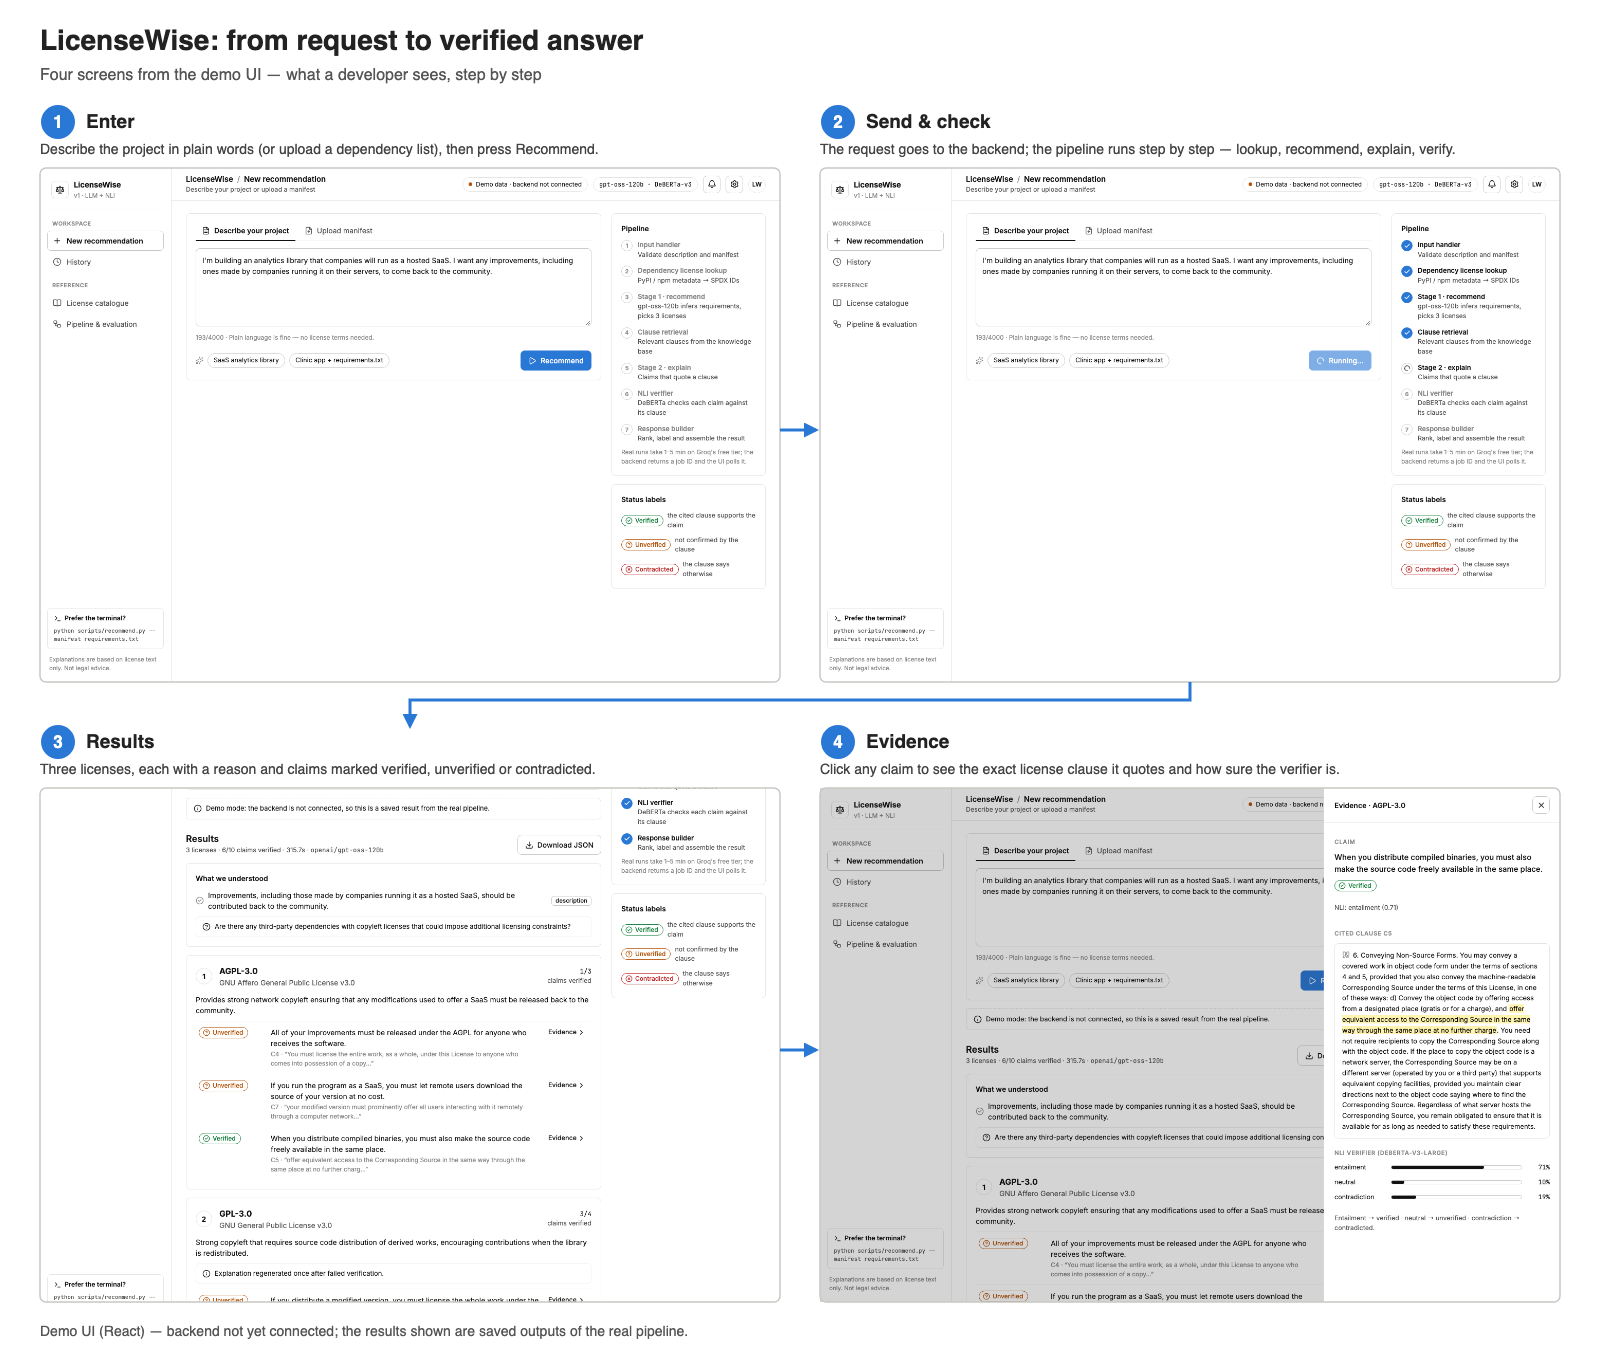
\includegraphics[width=0.92\textwidth]{22_ui_storyboard.png}
    \caption{User interface flow: (1) enter a description or manifest, (2) the pipeline runs, (3) results with verified/unverified/contradicted claims, (4) evidence drawer with the highlighted clause and NLI probabilities.}
    \label{fig:ui}
\end{figure*}

\paragraph{Implementation.}
The pipeline is a Python package (\texttt{licensewise}) with one module per step. All LLM calls request output that conforms to a JSON schema defined with Pydantic; the Stage~1 schema restricts license identifiers to the 34 catalogue entries and requires exactly three recommendations, and a duplicate recommendation triggers one retry. Stage~2 is re-run once, with the failed claims listed, if more than half of a license's claims fail verification. The web UI is built with React, TypeScript, and Vite. Data preparation and evaluation are reproducible scripts, and a Jupyter notebook reproduces every figure and result in this report.

\subsection{Machine Learning}
\label{ss:ml}

\begin{table}[tb]
    \caption{Models used in Phase 1. No model was fine-tuned.}
    \label{tab:models}
    \small
    \begin{tabularx}{\columnwidth}{@{}p{2.3cm}X@{}}
        \toprule
        \textbf{Model} & \textbf{Role and rationale} \\
        \midrule
        gpt-oss-120b (open-weight, via Groq~\cite{groq}) & Stage~1 recommendation and Stage~2 explanation. Maps informal intent to license concepts; strict JSON-schema output; free tier. \\
        DeBERTa-v3-large NLI~\cite{he2023debertav3,laurer2024less} & Verifier. Pre-trained by its authors on MNLI, FEVER-NLI, ANLI, LingNLI, and WANLI; used as-is, locally. Independent of the LLM. \\
        RoBERTa-large-MNLI~\cite{liu2019roberta} & Baseline verifier for RQ2. \\
        Qwen3.8-27B (via Groq) & Writes test descriptions (evaluation only). \\
        gpt-oss-20b (via Groq) & Checks test descriptions blind (evaluation only). \\
        \bottomrule
    \end{tabularx}
\end{table}

Table~\ref{tab:models} lists the models. The recommender and explainer use \textbf{gpt-oss-120b}, an open-weight model served through the Groq API. It is used \emph{zero-shot}: it receives instructions and the license catalogue but no examples and no task-specific training. An LLM is needed because translating informal preferences into license concepts such as copyleft or network-use clauses requires language understanding that fixed rules cannot provide.

The verifier is \textbf{DeBERTa-v3-large} fine-tuned for NLI by its authors on several public corpora~\cite{laurer2024less}; we did not train it. For each claim, the cited clause is the \emph{premise} and the claim is the \emph{hypothesis}; the model outputs probabilities for entailment, neutral, and contradiction, and the highest becomes the user-facing status (verified, unverified, contradicted). Before the NLI call, a quote check confirms that the quoted text appears verbatim in the cited clause; if not, the claim is marked unverified. An independent verifier is valuable because it does not share the LLM's errors, and its outputs double as an automatic faithfulness measure. We selected DeBERTa over a RoBERTa-large-MNLI baseline on the basis of RQ2 (Section~\ref{ss:rq2}).

Two further models are used only to build test data: Qwen3.8-27B writes project descriptions and gpt-oss-20b validates them. Using different models from the one under test reduces the risk that the system is evaluated on its own phrasing.

\subsection{Changes Since the Proposal}
\label{ss:changes}

The proposal described a fuller neuro-symbolic design with a rules engine, retrieval over a vector store, repository scanning, and fine-tuned models, with a hosted commercial LLM and validation by domain experts. Phase~1 deliberately implements a smaller core (v1) that can be built and evaluated end to end: an open-weight LLM via a free API instead of a hosted commercial model; selection of relevant clauses by keyword matching instead of vector retrieval, because full license texts exceed the free tier's per-minute token limit; registry metadata instead of repository scanning; no fine-tuning; and expert-free ground truth from curated public data. The rules engine and compatibility matrix are deferred to Phase~2, and the results below indicate that they are needed.
